\section{Data Sources and Reduction}
\label{sec:data}


\subsection{Data Sources}
\label{sec:sources}
In this study, we rely heavily on data from the \allwise\, extension of the \wise\, survey, combining data from the initial All-Sky Data Release, the 3-band cryogenic data release, and the NEOWISE post-cryogenic data release \citep{2013wise.rept....1C}. The initial \wise\,All-Sky Data Release observed the sky between January and August 2010, observing the sky 1.2 times with four detectors, operating at 3.4, 4.6, 12, and 22$\mu$m. Hereon we refer to \allwise\, photometric bands at [3.4$\mu$m/4.6$\mu$m/12$\mu$m/22$\mu$m] as [$W1/W2/W3/W4$]. The positions of objects in the \wise\, catalog were calibrated to the \twomass\, point source catalog. The 3-band cryogenic data release contains data from $W1$, 2, and 3, and surveyed $30\%$ of the sky between August and October 2010. During the 3-band cryogenic survey, $W1$ and $W2$ operated with nearly the same sensitivity as during the full survey. Warming of the telescope reduced sensitivity in $W3$ and fully saturated $W4$. The NEOWISE post-cryogenic data release contains $W1$ and $W2$ measurements, with sensitivities close to those obtained during the full cryogenic phase. During this phase, \wise\, surveyed $70\%$ of the sky. Data products from the post-cryogenic release included updated instrumental, astrometric, and photometric calibrations and reduction algorithms, resulting in much lower SNR. The overall number of sources compiled into \allwise\, totals over 747.6 million.

In order to generate a reliable, high-confidence catalog of Galactic candidate \agb\, stars, we must first define color-color criteria from known \agb\, star samples. We select \agb\, stars from three source catalogs: the {\it Optical Gravitational Lens Experiment-III Variable Star Catalog} \citep[\ogle,][]{2008AcA....58...69U,2009AcA....59..239S,2011AcA....61..217S}, the {\it MAssive Compact Halo Objects} project \citep[\macho,][]{1997ApJ...482...89A}, and the \simbad\, Astronomical Database \citep{2000A&AS..143....9W}. 

\ogle\, photometry for Long-Period Variables (LPVs) in the Small and Large Magellanic Clouds (SMC and LMC respsectively) was obtained between July 2001 and May 2009, with stars in the central 4.5-deg$^2$ of the LMC and SMC having an additional 5 observing seasons of photometry from OGLE-II. O-rich and C-rich \agb\, stars in \ogle\, were photometrically selected using reddening-free Wesenheit magnitudes, described in detail in \cite{2009AcA....59..239S,2011AcA....61..217S}. {\color{red}[Describe the selection bit in a little more detail, along with their sample completeness, selection biases, and contamination fractions]} Data reduction techniques are described in \cite{2008AcA....58...69U}. The resulting samples yield 46,467 \agb\, stars from the LMC (37,203 O-rich; 9,264 C-rich) and 6,509 stars from the SMC (3,727 O-rich; 2,782 C-rich). 

From \macho\, we obtain the sample of SMC, LMC, and Galactic Bulge AGB stars used in \cite{2008AJ....136.1242F} (14,861 stars). {\color{red}Why were these objects selected? Howe were they selected? What is their completeness, selection bias, and contamination fraction?} Following \cite{2008AJ....136.1242F}, the objects are divided into sequences (seq) 1-4. Sequence 1 primarily contains Mira variables pulsating in their fundamental modes, whereas Sequences 2-4 contain semi-regular variables in various pulsation modes.

The sample of AGB stars from \simbad\, was obtained by querying all objects classified as C-stars (18,656), S-stars (1,108), OH/IR stars (825), AGB stars (2,359), and Mira variables (9,608), for a total of 32,556 stars. Objects are classified spectroscopically, though by a variety of methods owing to the heterogeneous data housed within \simbad. Together with \macho\, and \ogle, the total sample of \agb\, stars is 100,393. Because there is a high likelihood that samples between \ogle, \macho, and \simbad overlap, we retain only unique objects after the initial data reduction in section~\ref{sec:reduction}.

We use \sdss\, spectroscopic catalogs to find and quantify regions in NIR-MIR color-color space populated by plausible contaminant sources. These include any Galactic stellar objects and planetary nebulae, as well as a host of extragalactic sources. Data for active galactic nuclei (AGN; 19,184 objects), quasi-stellar objects (QSOs; 122,550 objects), and star forming/burst galaxies (820,272 objects total) were drawn from \sdss\, DR7, specifically from the NYU Value Added Galaxy Catalog\footnote{\url{http://sdss.physics.nyu.edu/vagc/}} \citep[VAGC]{2005AJ....129.2562B}. Luminous Red Galaxies (LRGs) were selected from the SDSS Luminous Red Galaxy Survey \citep[105,631 objects, ][]{2010ApJ...710.1444K}.  Data for stars in the SDSS stellar locus were drawn from the DR 9 SEGUE Stellar Parameters Pipeline (SSPP) \citep[1,843,190 objects, ][]{2012ApJS..203...21A}. {\color{red} Include bit about YSOs and PNe from SIMBAD}

\subsection{Data Reduction}
\label{sec:reduction}
We use NASA/IPAC IRSA's {\tt GATOR} tool\footnote{\url{http://irsa.ipac.caltech.edu/cgi-bin/Gator/nph-scan?mission=irsa&submit=Select&projshort=WISE}} to positionally match \sdss, \ogle, \macho, and \simbad\, to \allwise. We select only matches within 3" between  each sample and \allwise. All samples of \agb\, were required to be brighter than the published 5$\sigma$ faint limits of [16.83/15.6/11.32/8.0], as well as fainter than the saturation limits of [2.0/1.5/-3.0/-4.0] extrapolated from the wings of the PSFs for point sources, for [$W1/W2/W3/W4$] \citep{2013wise.rept....1C}, with no flags for confusion or contamination as a spurious source in any band. We also require only single associations with \twomass\, objects within 3", detections in [$J/K_S/W1/W2/W3/W4$], and SNR $>$ 3 in each \allwise\, band. 

The population for each sample from initial matching as well as after the application of the \allwise\, faint limits, saturation limits, and \twomass\, detection requirements are shown in Table~\ref{tab:pop}. The WISE color-color distributions for the AGB and contaminant samples are shown in Figure~\ref{fig:distros}. \\

\vspace{-10pt}
%\begin{table}[h]
%	\begin{center}
%	\caption{AGB and Contaminant Populations}
%	\scalebox{0.85}{\begin{tabular}{l c c c c c c}
%		\hline
%		Population & SIMBAD C stars & OH/IR stars & Miras & S stars & AGB stars \\
%		\hline
%		2" match & 13,245 & 294 & 8,850 & 1,078 & 1,665 \\
%		Reduced & 3,327 & 165 & 6,218 & 865 & 1,121 \\
%		\hline\hline
%		Population & MACHO seq1 & seq2 & seq3 & seq4\\
%		\hline
%		2" match & 5,193 & 3,441 & 2,548 & 2,931 \\
%		Reduced & 927 & 642 & 263 & 336 \\
%		\hline\hline
%		Population & OGLE C-rich & O-rich\\
%		\hline
%		2" match & 11,417 & 38,369 \\
%		Reduced & 737 & 2515 \\
%		\hline\hline
%		Population & Locus Stars & AGN & LRG & QSO & Galaxies \\
%		\hline
%		2" match & 1,508,158 & 18,481 & 102,178 &  & 799,761 \\
%		Reduced & 168,045 & 9,652 & 7,717 & 18,360 & 125,869 \\
%		\hline
%
%		\label{tab:pop}
%	\end{tabular}}
%	\end{center}
%\end{table}

\begin{table}[h]
	\begin{center}
	
	\scalebox{0.85}{\begin{tabular}{l c c c c c c}
		\hline\hline
		Population & SIMBAD AGB* & C* & Mira & OH/IR & S* \\ 
		\hline
		3" match & 1,689 & 14,209 & 9,027 & 406 & 1,081 \\
		Reduced & 684 & 1,782 & 3,241 & 43 & 511 \\ 
		\hline
		Population & MACHO seq1 & seq2 & seq3 & seq4 \\ 
		\hline
		3" match & 5,279 & 3,519 & 2,619 & 3,070 \\
		Reduced & 277 & 185 & 73 & 61 \\ 
		\hline
		Population & OGLE-III C-rich & O-rich \\ 
		\hline
		3" match & 11,542 & 38,848 \\
		Reduced & 249 & 730 \\ 
		\hline
		Population & DR12 SSPP & DR7 LRG & QSO & AGN & Galaxies \\ 
		\hline
		3" match & 1,578,329 & 104,345 & 103,590 & 18,528 & 841,712 \\ 
		Reduced & 67,508 & 84 & 3,977 & 1,069 & 44,314 \\ 
		\hline\hline

		
	\end{tabular}}    
	\caption{\agb\, and contaminant populations matched to WISE before and after sample reduction in section~\ref{sec:reduction}. MACHO sequences (seq1-seq4) are from \cite{2008AJ....136.1242F} and described briefly in section~\ref{sec:sources}.\label{tab:pop}}
	\end{center}
	
\end{table}

\begin{figure}
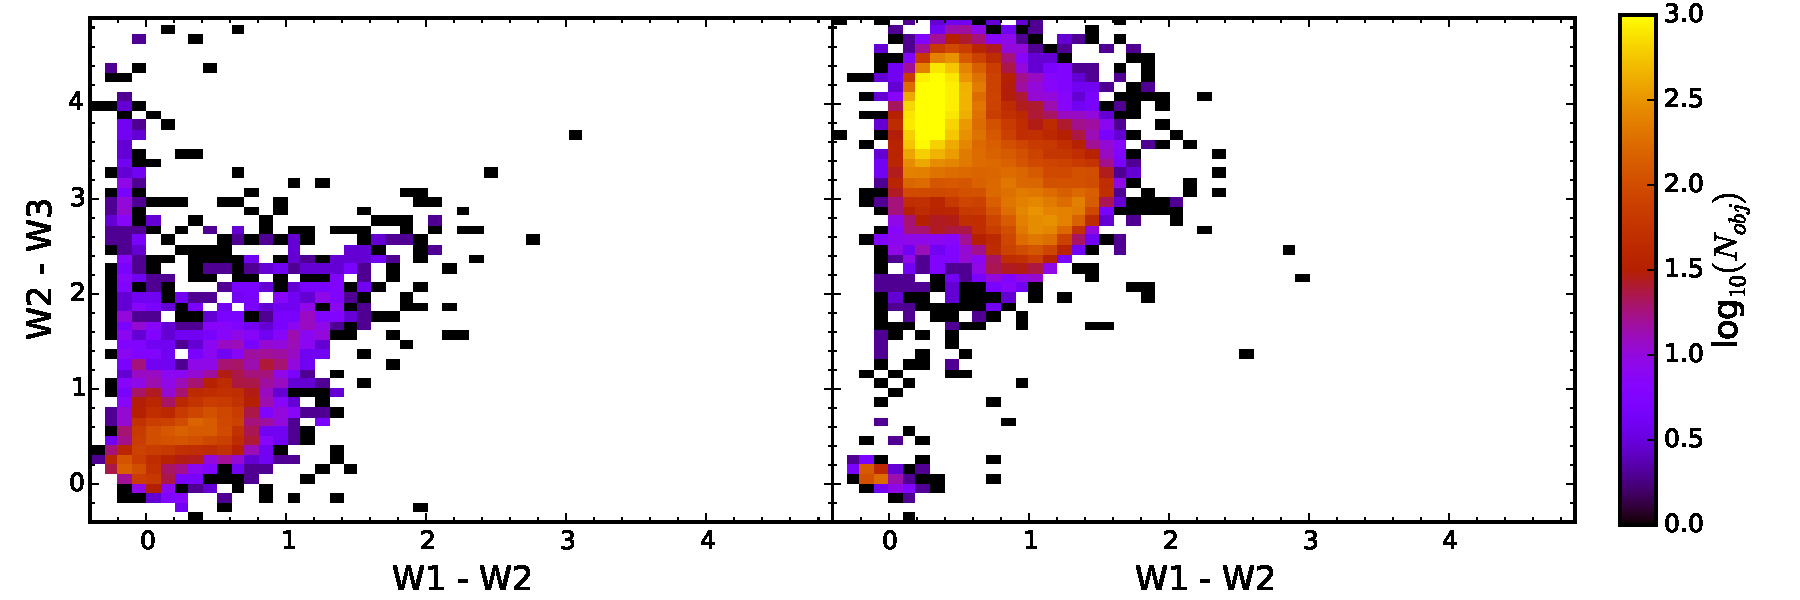
\includegraphics[width=7in]{figs/agbs_contaminants_color_color1.pdf}
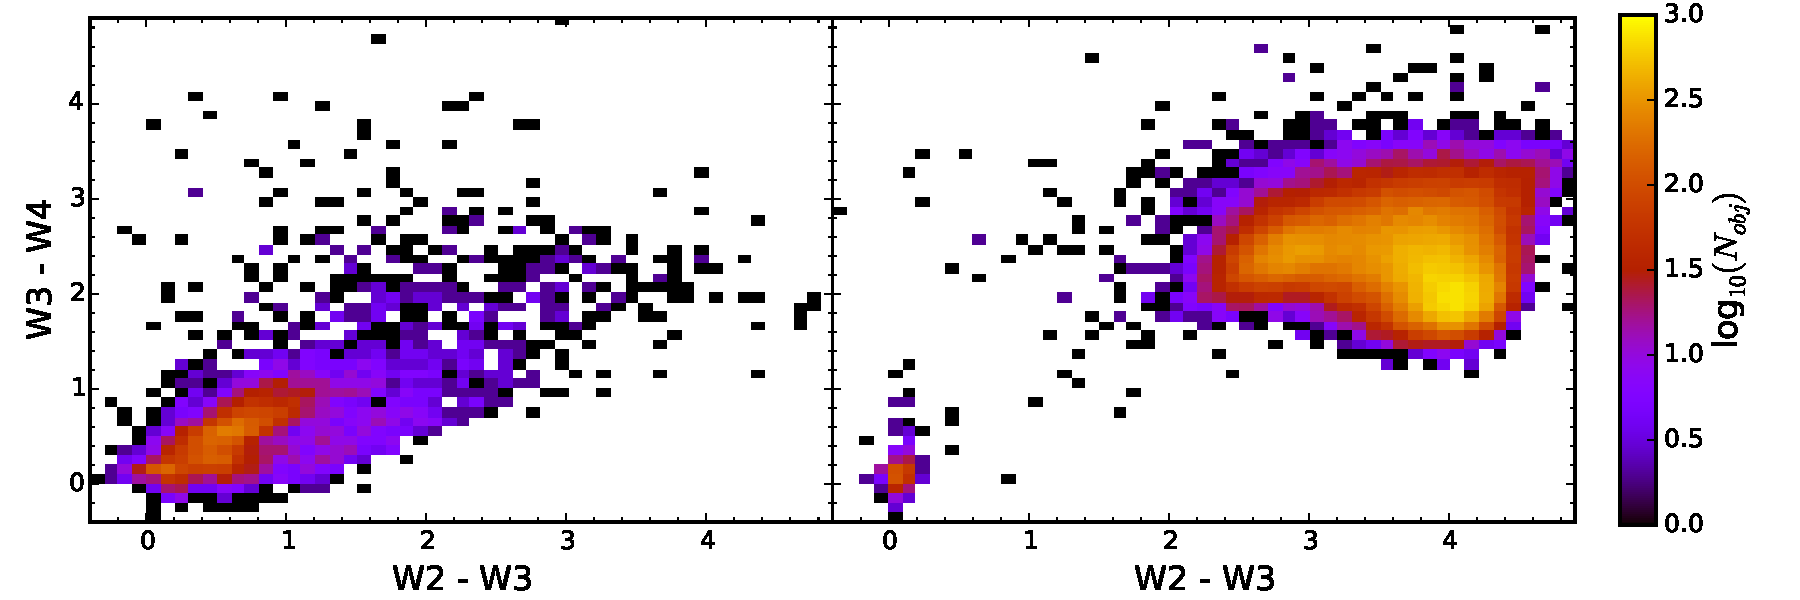
\includegraphics[width=7in]{figs/agbs_contaminants_color_color2.pdf}
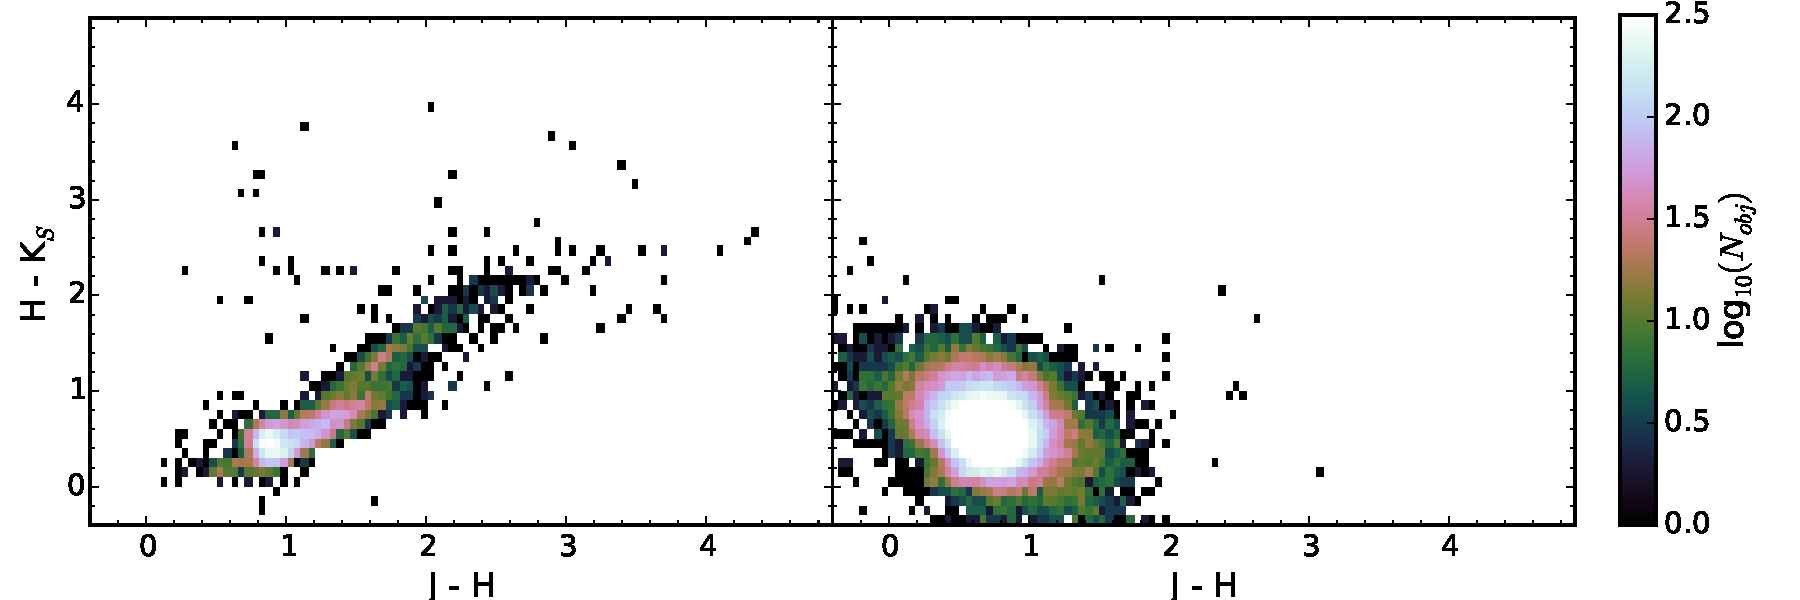
\includegraphics[width=7in]{figs/agbs_contaminants_color_color3.pdf}
\caption{Logarithmic number densities for objects in \wise\, and \twomass\, color-color space, binned in 0.1 dex on each axis. \emph{Left:} The combined AGB sample matched to ALLWISE. \emph{Right:} The combined contaminant sample.\label{fig:distros}}
\end{figure}

